% !TEX root=main.tex


\begin{appendices}

\section{Appendix A: MATLAB Code}

\label{appendix:A}



\subsection{Planning optimal path without constraints}

\lstinputlisting{code/ex23.m}



\subsection{LQ Controller}

\lstinputlisting{code/ex31.m}



\subsection{Planning optimal path with constraints}

\lstinputlisting{code/e4.m}

\lstinputlisting{code/confun.m}





\section{Appendix B: Simulink diagrams}

\label{appendix:B}

\begin{figure}[H]
    \centering
    \makebox[\textwidth][c]{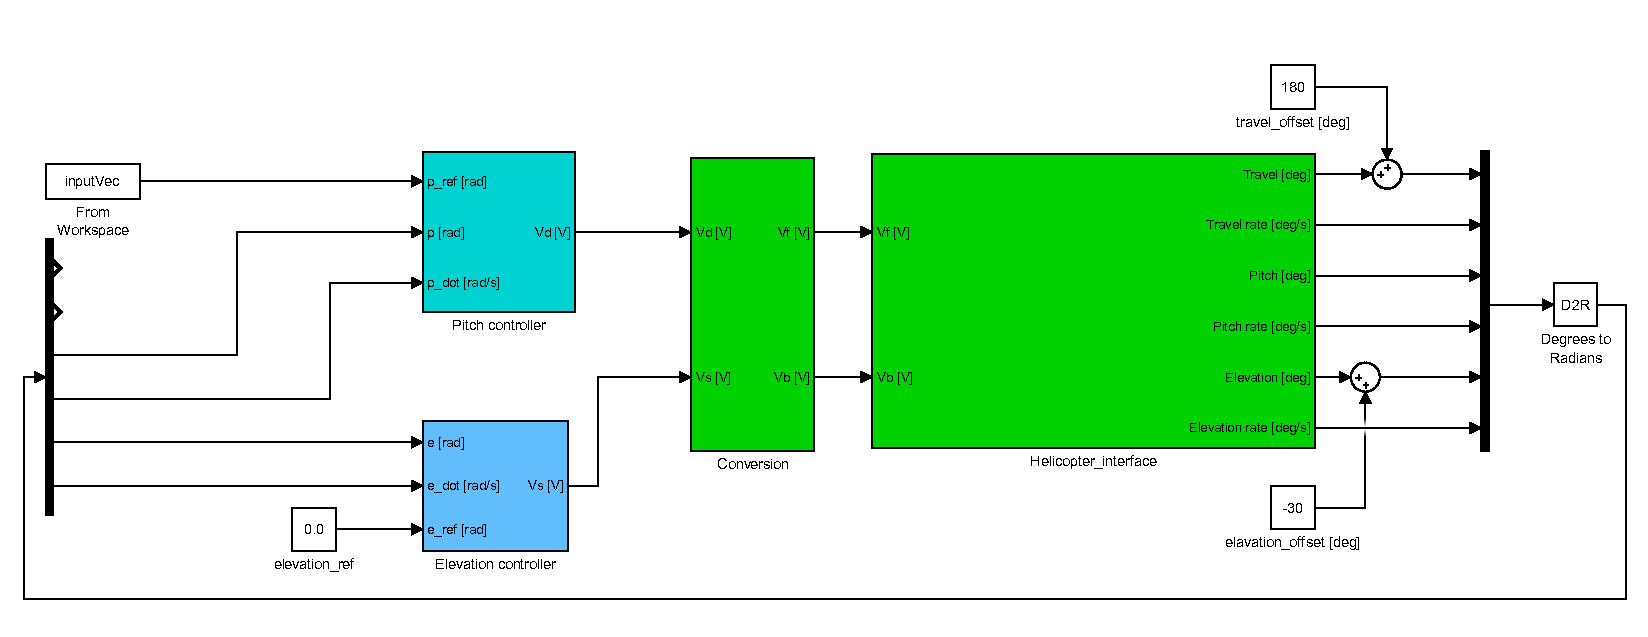
\includegraphics[width=1\textwidth]{E24_Cosmetic}}
    \caption{Simulink implementation of Ex.1.4.}
    \label{sim:ex24}
\end{figure}

\begin{figure}[H]

    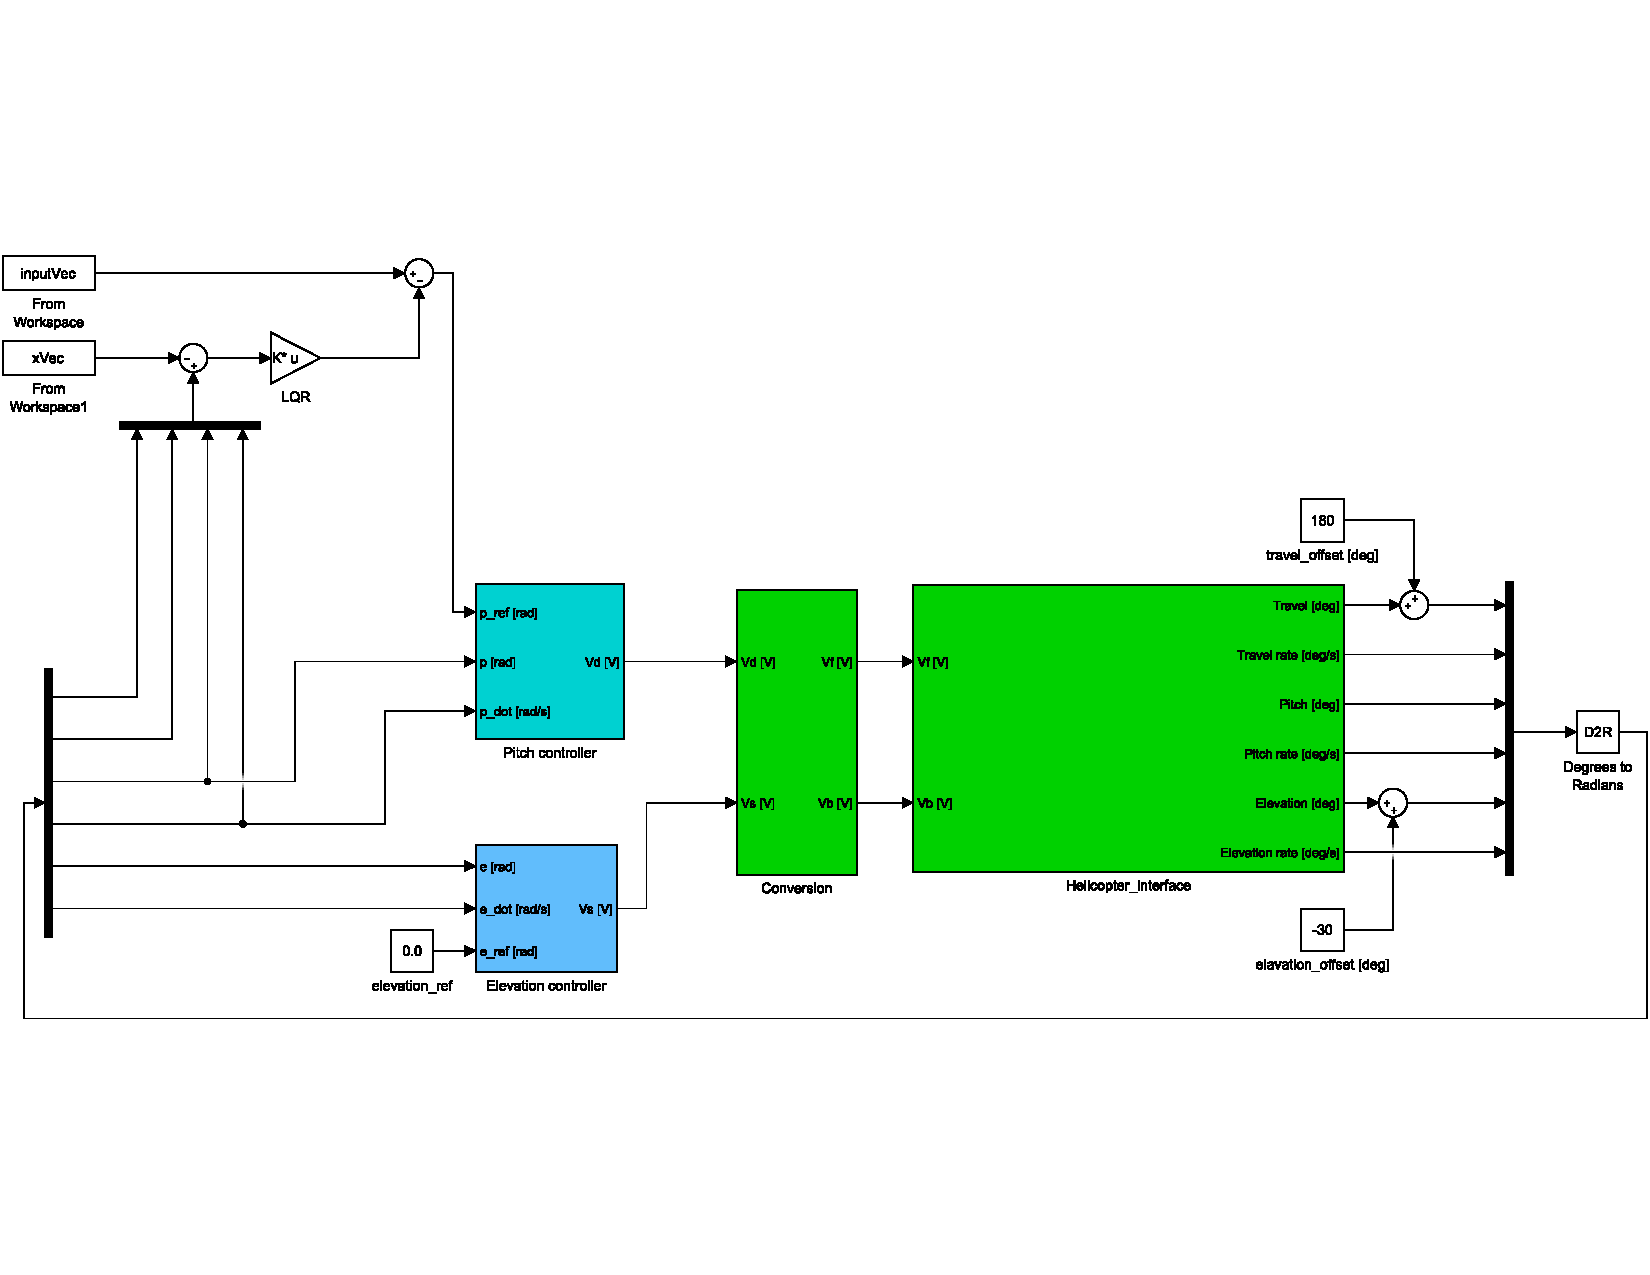
\includegraphics[width=\textwidth]{ex3sim.pdf}

    \caption{Simulink diagram used in exercise 3 including LQ controller}

    \label{fig:simulink_LQ}

\end{figure}

\begin{figure}[H]

    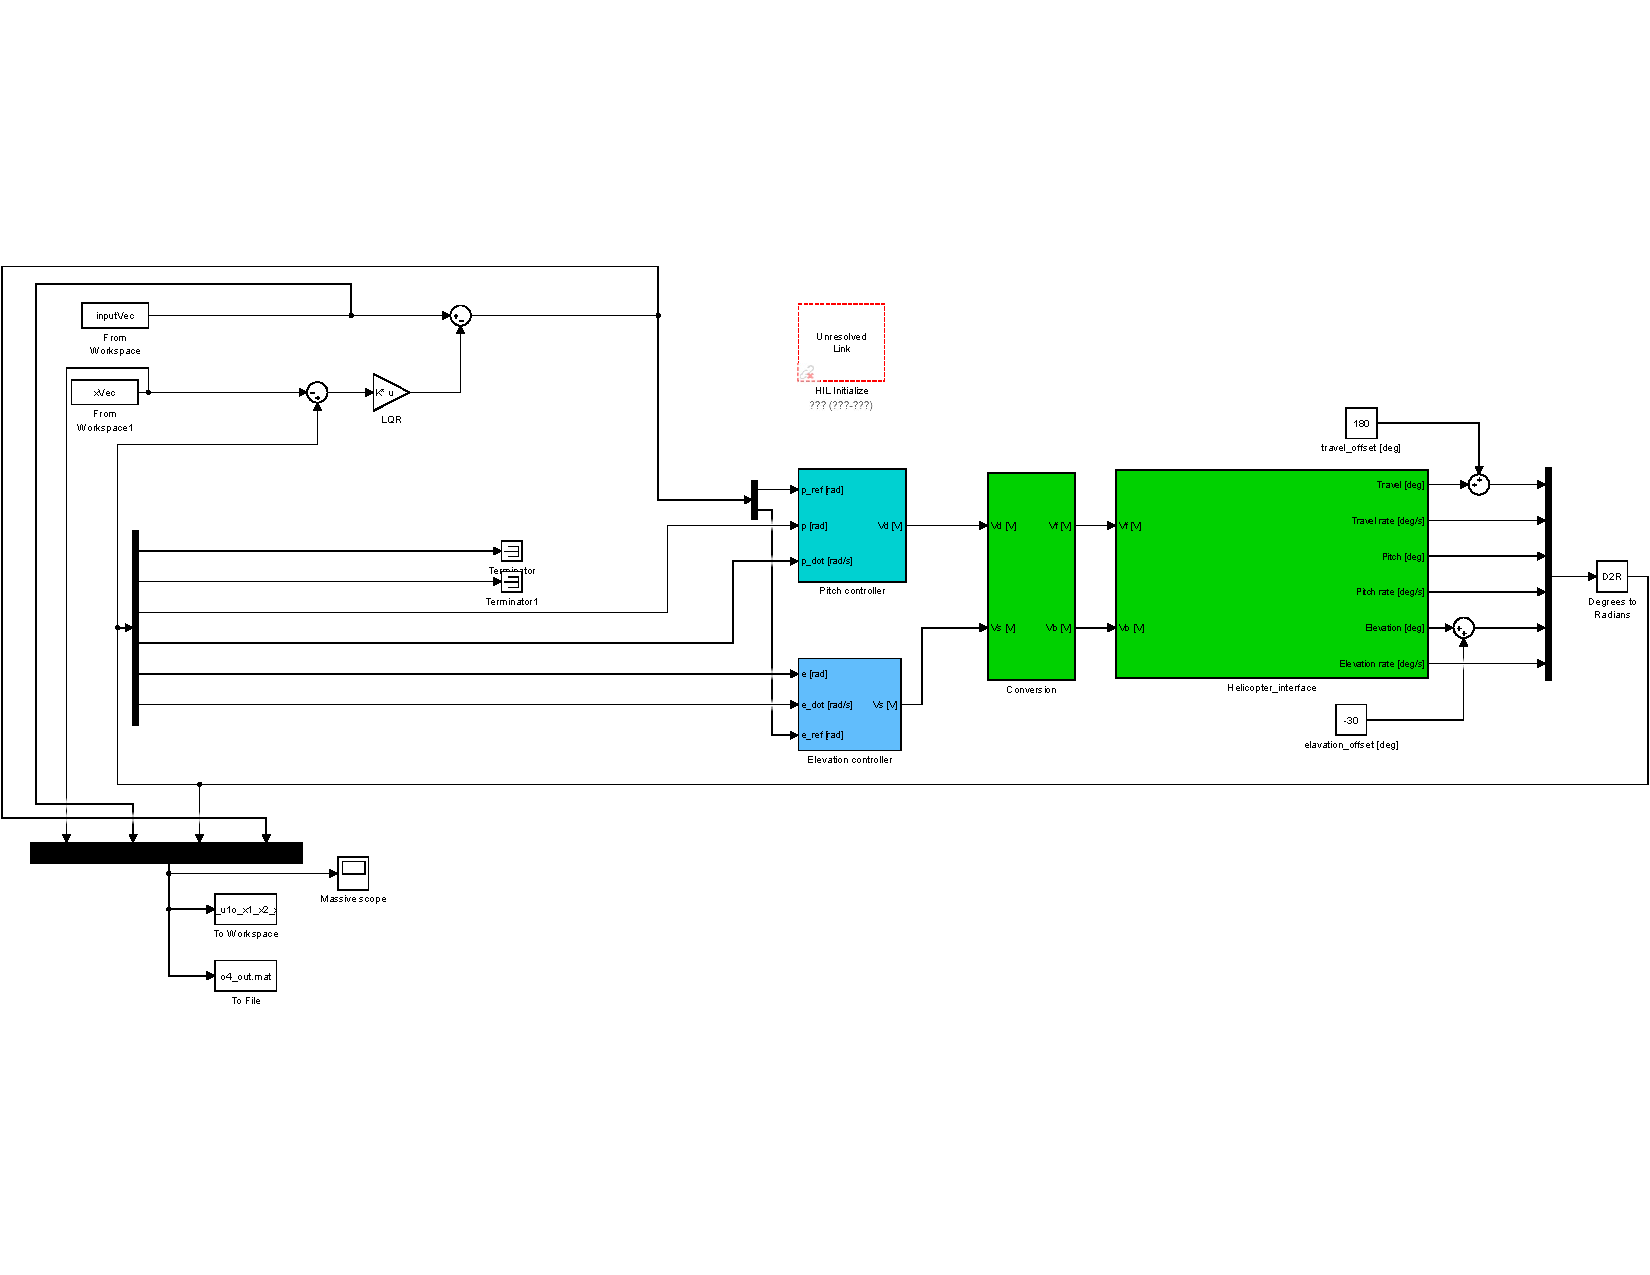
\includegraphics[width=\textwidth]{ex4sim.pdf}

    \caption{Simulink diagram used in exercise 4. The ``LQR'' multiplication block output was disconnected when feedback was not wanted.}

\end{figure}

\end{appendices}
